% Created 2022-11-16 mer 14:34
% Intended LaTeX compiler: pdflatex
\documentclass[presentation]{beamer}
\usepackage[utf8]{inputenc}
\usepackage[T1]{fontenc}
\usepackage{graphicx}
\usepackage{longtable}
\usepackage{wrapfig}
\usepackage{rotating}
\usepackage[normalem]{ulem}
\usepackage{amsmath}
\usepackage{amssymb}
\usepackage{capt-of}
\usepackage{hyperref}
\usepackage{minted}
\usepackage[, french]{babel}
\usepackage{svg}
\logo{
\includegraphics[width=.1\textwidth]{../../by-sa.png}}
\usetheme{metropolis}
\usecolortheme{}
\usefonttheme{}
\useinnertheme{}
\useoutertheme{}
\author{Guy Bégin}
\date{\today}
\title{Circuits logiques combinatoires et séquentiels}

\hypersetup{
 pdfauthor={Guy Bégin},
 pdftitle={Circuits logiques combinatoires et séquentiels},
 pdfkeywords={},
 pdfsubject={},
 pdfcreator={Emacs 28.1 (Org mode 9.5.4)}, 
 pdflang={French}}
\begin{document}

\maketitle

\section{Circuits séquentiels}
\label{sec:org621d0f7}

\begin{frame}[label={sec:org099e9b7}]{Objectifs}
\begin{itemize}
\item Pouvoir identifier un circuit logique séquentiel
\item Savoir distinguer entre les circuits séquentiels synchrones et asynchrones
\item Être familier avec les principaux types de loquets, pouvoir en
expliquer le fonctionnement
\item Être familier avec les principaux types de bascules, pouvoir en
expliquer le fonctionnement
\end{itemize}
\end{frame}

\begin{frame}[label={sec:orgd96dbf8}]{Modèle d'un circuit séquentiel}
\begin{itemize}
\item Les circuits logiques séquentiels sont ceux qui comportent de la mémoire.

\item Le modèle général d'un circuit séquentiel est illustré sur la figure \ref{fig:org41949e9}.
\end{itemize}

\begin{figure}[htbp]
\centering
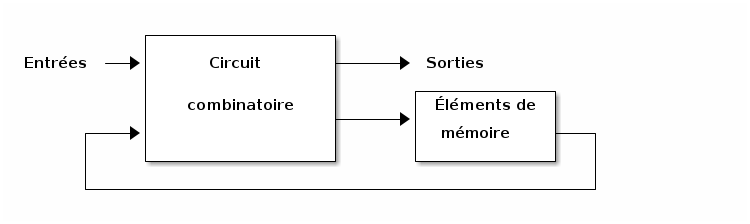
\includegraphics[width=.9\linewidth]{../../Sources_images_logiques/images/circuit_seq.png}
\caption{\label{fig:org41949e9}Modèle de circuit séquentiel}
\end{figure}
\end{frame}

\begin{frame}[label={sec:orgaed08f2}]{Modèle d'un circuit séquentiel \ldots{} 2}
\begin{itemize}
\item On y voit qu'il y a une boucle de rétroaction, qui fait que les valeurs binaires stockées dans les éléments de mémoire contribuent au calcul des sorties.

\item Les sorties du circuit à un instant donné ne dépendent donc pas seulement des entrées présentes à ce moment, mais aussi de ces valeurs qui sont mémorisées dans le système.

\item Pour décrire cette situation dans laquelle se trouvent les valeurs stockées en mémoire, on parle de l'\alert{état} du système.

\item Selon les entrées et l'état à un instant donné, le système pourra changer d'état selon les changements qui seront apportés par la portion combinatoire aux valeurs mémorisées.
\end{itemize}
\end{frame}

\begin{frame}[label={sec:orge49b2af}]{Modèle d'un circuit séquentiel \ldots{} 3}
\begin{itemize}
\item On verra donc le système évoluer au fil du temps, passant d'un état à un autre, et générant des sorties en fonction des entrées et de l'état du moment.

\item Intuitivement, on peut penser que le nombre d'états distincts sera fonction du nombre de valeurs binaires qui seront mémorisées.

\item Le comportement d'un système séquentiel est donc caractérisé par une séquence temporelle d'entrées, de sorties et de valeurs interne d'état.
\end{itemize}
\end{frame}

\begin{frame}[label={sec:org135c244}]{Circuits séquentiel synchrones ou asynchrones}
\begin{itemize}
\item On peut distinguer les circuits séquentiels selon la relation de synchronisation qui existe entre les différents signaux du système.

\item Dans un circuit séquentiel \alert{synchrone}, le comportement du système peut se définir en fonction des valeurs de ses signaux à des instants discrets prédéterminés.

\item Le comportement d'un circuit séquentiel \alert{asynchrone} dépend à tout moment des signaux d'entrée et de l'ordre dans lequel ces signaux changent.
\end{itemize}
\end{frame}

\begin{frame}[label={sec:orgd781935}]{Circuits séquentiel synchrones}
\begin{itemize}
\item Un circuit séquentiel synchrone fait appel à un signal spécial appelé \alert{horloge} qui rythme les changement d'état et de sorties afin qu'il se produisent à des instants discrets.

\item Les éléments de mémoire qui stockent les valeurs binaires sont appelés \alert{bascules} (\emph{flip-flops} en anglais).

\item Il existe différents types de bascules.

\item Nous les étudierons en détail, car elles sont à la base des circuits séquentiels les plus utilisés.
\end{itemize}
\end{frame}

\begin{frame}[label={sec:orgba4412c}]{Modèle de circuit séquentiel synchrone}
\begin{itemize}
\item La figure suivante présente le modèle général d'un circuit séquentiel synchrone.
\end{itemize}

\begin{figure}[htbp]
\centering
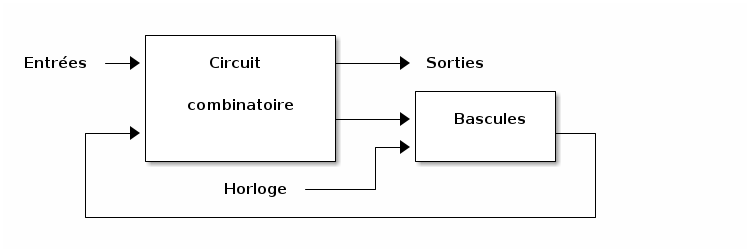
\includegraphics[width=.9\linewidth]{../../Sources_images_logiques/images/circuit_seq_sync.png}
\caption{\label{fig:orgbbc7650}Modèle de circuit séquentiel synchrone}
\end{figure}
\end{frame}

\begin{frame}[label={sec:org21885ac}]{Signal d'horloge}
\begin{itemize}
\item Le signal d'horloge est typiquement une onde carrée, telle qu'illustré sur la figure suivante.
\end{itemize}

\begin{figure}[htbp]
\centering
\includesvg[width=.9\linewidth]{../../Sources_images_logiques/images/horloge}
\caption{\label{fig:orge6d4e62}Signal d'horloge}
\end{figure}
\end{frame}

\begin{frame}[label={sec:org795c356}]{Éléments de mémoire}
\begin{itemize}
\item Un élément de mémoire peut maintenir son état binaire indéfiniment (à condition, évidemment, qu'il soit alimenté).

\item Son état est observable par l'intermédiaire de ses sorties.

\item On doit agir via la ou les entrées de l'élément pour le faire changer d'état.

\item Les différents types d'éléments de mémoire sont caractérisés par le nombre et le type d'entrées.
\end{itemize}
\end{frame}

\begin{frame}[label={sec:org6497c6a}]{Éléments de mémoire \ldots{} 2}
\begin{itemize}
\item Les éléments de mémoire qui sont contrôlés par les niveaux de leurs entrées sont appelés des \alert{loquets} (\emph{latches} en anglais).

\item Les éléments contrôlés par des changements ou \alert{transitions} de niveaux sont appelés des bascules.

\item Les transitions sont appliquées à une entrée spéciale d'horloge qui sert à déclencher les changements d'état à des instants précis.

\item Les loquets sont des ingrédients de base dans la conception des bascules.

\item Nous les étudierons en premier.
\end{itemize}
\end{frame}


\begin{frame}[label={sec:org01d12e2},fragile]{Loquet SR}
 \begin{itemize}
\item Le loquet SR est formé de deux portes NOR interconnectées et comporte deux entrées: \(S\) pour \texttt{Set}, qui permet de mémoriser une valeur 1, et \(R\) pour \texttt{Reset}, qui permet de mémoriser une valeur 0.

\item Le schéma classique du loquet SR montré sur la figure \ref{fig:org917612e} ne fait pas ressortir la boucle de rétroaction, mais si on déplace un peu les éléments sans changer les connexions, on voit mieux le lien de retour caractéristique de la boucle.

\item Sur la figure \ref{fig:orge298dd8}, la porte reliée à \(S\) a été placée devant, mais nous aurions pu tout aussi bien mettre l'autre porte en avant.

\item Aucune des deux n'est vraiment devant l'autre, puisqu'il s'agit d'une boucle n'ayant ni début ni fin.
\end{itemize}
\end{frame}

\begin{frame}[label={sec:org291a86e}]{Loquet SR \ldots{} 2}
\begin{figure}[htbp]
\centering
\includesvg[scale=0.75]{../../Sources_images_logiques/images/SRlatch}
\caption{\label{fig:org917612e}Schéma du loquet SR avec portes NOR}
\end{figure}
\end{frame}

\begin{frame}[label={sec:org56a31d6}]{Loquet SR \ldots{} 3}
\begin{figure}[htbp]
\centering
\includesvg[scale=0.75]{../../Sources_images_logiques/images/SRlatch_bouc}
\caption{\label{fig:orge298dd8}Schéma du loquet SR NOR mettant la boucle en évidence}
\end{figure}
\end{frame}

\begin{frame}[label={sec:orgd50fbb0},fragile]{Loquet SR \ldots{} 4}
 \begin{itemize}
\item Quand les sorties sont \(Q=1, Q^\prime=0\), on dit que le loquet est dans l'état activé (\texttt{set}).

\item Lorsque \(Q=0, Q^\prime=1\), le loquet est désactivé (\texttt{reset}).

\item Les sorties \(Q\) et \(Q^\prime\) sont normalement complémentaires.

\item Si on active la condition d'entrée \(S=1, R=1\), les deux sorties seront à 0, mais lorsqu'on relâchera les entrées, le loquet passera à un état imprévisible, voire instable.
\end{itemize}
\end{frame}

\begin{frame}[label={sec:org6b5bbe3}]{Loquet SR \ldots{} 5}
\begin{itemize}
\item Dans une application normale, on voudra éviter la cas d'entrée \(S=1, R=1\).

\item En fonctionnement normal, à moins de vouloir changer l'état, on garde les deux entrées à \(S=0, R=0\) et l'état du loquet se maintient.

\item En appliquant le niveau 1 pendant un certain temps à \(S\) seulement, le loquet s'active, peu importe l'état dans lequel il se trouvait auparavant.
\end{itemize}
\end{frame}

\begin{frame}[label={sec:orge39d632}]{Loquet SR \ldots{} 6}
\begin{itemize}
\item On doit s'assurer de ramener l'entrée \(S\) à 0 avant d'effectuer d'autres changements aux entrées, pour éviter le cas interdit \(S=1, R=1\).

\item De même, en appliquant le niveau 1 pendant un certain temps à \(R\) seulement, le loquet se désactive, peu importe l'état dans lequel il se trouvait auparavant.
\end{itemize}
\end{frame}

\begin{frame}[label={sec:orgc0086b5}]{Loquet SR: tableau de fonctionnement}
\begin{table}[htbp]
\caption{\label{tab:org2086ad1}Loquet SR NOR: tableau de fonctionnement}
\centering
\begin{tabular}{rrlrrl}
\(S\) & \(R\) &  & \(Q\) & \(Q^\prime\) & \\
\hline
1 & 0 &  & 1 & 0 & \\
0 & 0 &  & 1 & 0 & après \(s=1, R=0\)\\
0 & 1 &  & 0 & 1 & \\
0 & 0 &  & 0 & 1 & après \(s=0, R=1\)\\
1 & 1 &  & 0 & 0 & interdit\\
\end{tabular}
\end{table}
\end{frame}

\begin{frame}[label={sec:org58c67d2}]{Loquet SR avec portes NAND}
\begin{itemize}
\item On peut aussi concevoir un loquet avec des portes NAND, comme sur la figure \ref{fig:orgf1a3b75}.
\end{itemize}

\begin{figure}[htbp]
\centering
\includesvg[scale=0.75]{../../Sources_images_logiques/images/SRlatch_nand}
\caption{\label{fig:orgf1a3b75}Loquet SR en portes NAND}
\end{figure}
\end{frame}

\begin{frame}[label={sec:org46962dd}]{Loquet SR avec portes NAND \ldots{} 2}
\begin{itemize}
\item Le fonctionnement est sensiblement le même, si ce n'est que les niveaux sont inversés par rapport au loquet NOR comme on peut le voir sur le tableau de fonctionnement (tableau \ref{tab:org2c7b0c7}).

\item Par exemple, on garde les deux entrées à \(S=1, R=1\) pour maintenir l'état du loquet.
\end{itemize}
\end{frame}

\begin{frame}[label={sec:orgcdde014}]{Loquet SR NAND: tableau de fonctionnement}
\begin{table}[htbp]
\caption{\label{tab:org2c7b0c7}Loquet SR NAND: tableau de fonctionnement}
\centering
\begin{tabular}{rrlrrl}
\(S\) & \(R\) &  & \(Q\) & \(Q^\prime\) & \\
\hline
1 & 0 &  & 0 & 1 & \\
1 & 1 &  & 0 & 1 & après \(s=1, R=0\)\\
0 & 1 &  & 1 & 0 & \\
1 & 1 &  & 1 & 0 & après \(s=0, R=1\)\\
0 & 0 &  & 1 & 1 & interdit\\
\end{tabular}
\end{table}
\end{frame}

\begin{frame}[label={sec:org7b59088}]{Loquet avec signal de contrôle}
\begin{itemize}
\item On peut ajouter un signal de contrôle d'entrée \(E\) (\emph{enable}) pour contrôler \alert{quand} le loquet pourra être affecté par les signaux d'entrée.

\item Le circuit est représenté à la figure \ref{fig:orgbe37de0}.
\end{itemize}

\begin{figure}[htbp]
\centering
\includesvg[scale=0.75]{../../Sources_images_logiques/images/SRlatch_nand_en}
\caption{\label{fig:orgbe37de0}Loquet SR NAND avec signal de contrôle}
\end{figure}
\end{frame}

\begin{frame}[label={sec:org23cd420}]{Loquet avec signal de contrôle}
\begin{table}[htbp]
\caption{\label{tab:orgb91c010}Loquet SR avec signal de contrôle: tableau de fonctionnement}
\centering
\begin{tabular}{rrrll}
\(E\) & \(S\) & \(R\) &  & prochain \(Q\)\\
\hline
0 & X & X &  & inchangé\\
1 & 0 & 0 &  & inchangé\\
1 & 0 & 1 &  & \(Q = 0\)\\
1 & 1 & 0 &  & \(Q = 1\)\\
1 & 1 & 1 &  & indéterminé\\
\end{tabular}
\end{table}
\end{frame}

\begin{frame}[label={sec:org99cd461}]{Loquet avec signal de contrôle \ldots{} 2}
\begin{itemize}
\item Comme on peut voir dans le tableau \ref{tab:orgb91c010}, les sorties des portes NAND d'entrée demeurent à 1 tant que \(E = 0\), et le loquet ne peut pas être affecté par les entrées \(S\) et \(R\).

\item Quand on active \(E = 1\), le circuit peut être actionné par les entrées \(S\) et \(R\).

\item La condition pour activer est \(S=1, R=0\); pour désactiver, c'est \(S=0, R=1\).

\item Lorsque \(E = 1\), on ne doit pas faire \(S=1, R=1\), car on mettrait le loquet dans un état indéterminé.

\item Le loquet SR avec contrôle est surtout important comme ingrédient de base pour la conception de bascules.
\end{itemize}
\end{frame}

\begin{frame}[label={sec:org72559af}]{Loquet D}
\begin{itemize}
\item Une option pour éliminer la condition qui fait apparaître un état indéterminé est de s'assurer de toujours commander \(S\) et \(R\) avec des signaux complémentaires.

\item C'est ainsi qu'on arrive au loquet D, illustré sur la figure \ref{fig:orga6e4afc}, qui ne comporte qu'une entrée de données \(D\) et une entrée de contrôle \(E\).

\item La valeur de \(D\) est reflétée à \(Q\) lorsque \(E=1\) et se maintient après que \(E\) passe à 0 (tableau \ref{tab:org24c2479}).
\end{itemize}
\end{frame}

\begin{frame}[label={sec:org0af315e}]{Loquet D: schéma}
\begin{figure}[htbp]
\centering
\includesvg[scale=0.75]{../../Sources_images_logiques/images/Dlatch}
\caption{\label{fig:orga6e4afc}Schéma du loquet D}
\end{figure}
\end{frame}

\begin{frame}[label={sec:org5afbbb3}]{Loquet D: tableau de fonctionnement}
\begin{table}[htbp]
\caption{\label{tab:org24c2479}Loquet D: tableau de fonctionnement}
\centering
\begin{tabular}{rrll}
\(E\) & \(D\) &  & prochain \(Q\)\\
\hline
0 & X &  & inchangé\\
1 & 0 &  & \(Q = 0\)\\
1 & 1 &  & \(Q = 1\)\\
\end{tabular}
\end{table}
\end{frame}

\begin{frame}[label={sec:org5026759}]{Loquet D: symbole}
\begin{itemize}
\item Le symbole graphique d'un loquet D est illustré à la figure suivante.
\end{itemize}

\begin{figure}[htbp]
\centering
\includesvg[scale=0.75]{../../Sources_images_logiques/images/schema_latchD}
\caption{\label{fig:org843a0fe}Symbole du loquet D}
\end{figure}
\end{frame}

\begin{frame}[label={sec:org743f455}]{Application: rebonds d'interrupteurs}
\begin{itemize}
\item Lorsqu'on utilise un interrupteur pour commuter un signal entre les niveaux qui correspondent aux valeurs logiques 0 et 1, le contact ne se fait pas de façon franche sans hésitations, et le signal observé rebondit plusieurs fois avant de se stabiliser à sa valeur, comme on peut le voir sur la partie de gauche de la figure \ref{fig:org5ed2c3b}.

\item Ces rapides aller-retours entre les niveaux peuvent bien souvent déclencher un circuit logique et le mettre dans un état imprévisible.
\end{itemize}
\end{frame}

\begin{frame}[label={sec:org718ca82}]{Contacts et rebonds}
\begin{figure}[htbp]
\centering
\includesvg[width=.9\linewidth]{../../Sources_images_logiques/images/debounce}
\caption{\label{fig:org5ed2c3b}Contacts et rebonds}
\end{figure}
\end{frame}

\begin{frame}[label={sec:org4310c5d}]{Application: loquet contre rebonds d'interrupteurs}
\begin{itemize}
\item Pour éviter ce problème, on peut faire appel à un loquet selon la configuration de la partie droite de la figure.

\item Le loquet réagit dès que l'entrée B passe à 0.

\item Même si cette entrée remonte à 1, la valeur \(Q\) est maintenue.

\item On obtient donc une transition franche sur \(Q\).
\end{itemize}
\end{frame}

\begin{frame}[label={sec:org7ef1799}]{Bascules (Flip Flops)}
\begin{itemize}
\item Les loquets peuvent remplir le rôle de mémoriser des valeurs binaires, mais le fait que les changements d'état soient activés par un \alert{niveau} pose des difficultés.

\item En effet, si les valeurs à l'entrée changent pendant que le signal de contrôle est actif, la valeur qui sera mémorisée par la rétroaction sera la dernière qui aura eu le temps de s'y établir, qui ne sera pas nécessairement la valeur que le concepteur voulait.

\item Si la sortie du loquet est acheminée, directement ou à travers un circuit combinatoire, vers ses entrées ou les entrées d'autres loquets (activés par le même signal de contrôle) dans une boucle du circuit séquentiel, il se peut que les délais de propagation et de prise en compte des entrées fassent que la sortie globale du circuit séquentiel soit imprévisible.
\end{itemize}
\end{frame}

\begin{frame}[label={sec:orge4e00f7}]{Bascules (Flip Flops) \ldots{} 2}
\begin{itemize}
\item La conception des bascules vise à corriger ce problème, en établissant un instant précis et prévisible de déclenchement où les valeurs d'entrée seront prises en compte systématiquement.

\item Le concept essentiel est que l'état d'une bascule est modifié uniquement au moment où il y a un changement dans son signal de contrôle.

\item Ce changement momentané est appelé \alert{transition} et on dit que c'est la transition qui provoque le changement d'état qui \alert{déclenche} la bascule.
\end{itemize}
\end{frame}

\begin{frame}[label={sec:org20d6ca0}]{Bascules et déclenchement}
\begin{itemize}
\item On parlera de déclenchement sur le \alert{front montant} lorsque la transition qui provoque le déclenchement passe d'un niveau bas vers un niveau élevé, et de déclenchement sur le \alert{front descendant} dans le cas d'une transition du haut vers le bas.

\item On illustre parfois le front de déclenchement au moyen d'une flèche, comme on peut le voir sur la figure \ref{fig:org755021d}.
\end{itemize}


\begin{figure}[htbp]
\centering
\includesvg[width=.9\linewidth]{../../Sources_images_logiques/images/horlogeP}
\caption{\label{fig:org755021d}Signaux d'horloge avec fronts de déclenchement}
\end{figure}
\end{frame}

\begin{frame}[label={sec:orgf5e9b88}]{Bascule D}
Le secret pour isoler la valeur mémorisée par l'élément de mémoire des changements qui pourraient survenir sur les entrées consiste à utiliser un mécanisme semblable à celui d'un sas.

Selon Larousse, la définition d'un sas est

\begin{quote}
Enceinte ou passage clos, muni de deux portes ou systèmes de fermeture
dont on ne peut ouvrir l'un que si l'autre est fermé et qui permet de
passer ou de faire passer d'un milieu à un autre en maintenant ceux-ci
isolés l'un de l'autre.
\end{quote}
\end{frame}

\begin{frame}[label={sec:orgd653ebb}]{Bascule D \ldots{} 2}
\begin{itemize}
\item Dans notre contexte, nous utiliserons deux loquets en série, avec la sortie du premier, appelé \alert{maître} reliée à l'entrée du deuxième, appelé \alert{esclave}.

\item Le loquet maître sera activé par le signal d'horloge alors que le loquet esclave sera activé par le complément du signal d'horloge.

\item De cette façon, un seul des loquets sera actif à la fois, comme dans un sas.

\item La figure \ref{fig:org1bef66f} illustre la configuration pour réaliser une bascule D maître-esclave.
\end{itemize}
\end{frame}

\begin{frame}[label={sec:org7752e28}]{Bascule D maître-esclave}
\begin{figure}[htbp]
\centering
\includesvg[scale=0.75]{../../Sources_images_logiques/images/D_mast_slave_sanst}
\caption{\label{fig:org1bef66f}Bascule D maître-esclave}
\end{figure}
\end{frame}

\begin{frame}[label={sec:org2bbb95f}]{Bascule D maître-esclave: fonctionnement}
\begin{itemize}
\item Lorsque le signal d'horloge est au niveau haut, seul le loquet maître pourra réagir au signal d'entrée.

\item Puis, lorsque le signal d'horloge sera au niveau bas, ce premier loquet sera désactivé, sa sortie sera maintenue, et le deuxième loquet sera activé.

\item Comme l'entrée du loquet esclave est alimentée par le loquet maître dont la sortie est maintenue, c'est la valeur mémorisée par le maître qui sera mémorisée dans l'esclave, et qui apparaîtra donc en sortie de l'ensemble.
\end{itemize}
\end{frame}

\begin{frame}[label={sec:org06e87bd}]{Bascule D maître-esclave: fonctionnement \ldots{} 2}
\begin{itemize}
\item La valeur qui sera ultimement mémorisée est celle qui se trouvait tout juste avant la transition de l'horloge passant du niveau haut vers le niveau bas.

\item Nous avons donc créé une bascule sensible au \alert{front descendant}.
\end{itemize}
\end{frame}

\begin{frame}[label={sec:orgbba4af7}]{Bascule D maître-esclave: fonctionnement \ldots{} 3}
En résumé:

\begin{enumerate}
\item La sortie \(Q\) ne changera qu'une seule fois par cycle d'horloge.
\item Un changement de valeur sera causé par la valeur d'entrée présente
juste avant le front descendant de l'horloge.
\item La valeur de sortie changera effectivement (s'il y a lieu) pendant
la demi-période basse de l'horloge.
\end{enumerate}
\end{frame}

\begin{frame}[label={sec:orgd6b8824}]{Autres configurations}
\begin{itemize}
\item D'autres configuations permettent de réaliser ce comportement de sas.

\item Par exemple, le circuit de la figure \ref{fig:org47f3cb0} utilise trois éléments en loquet SR NAND: les deux premiers sont activés par le signal de donnée \(D\) et l'horloge, et le dernier mémorise et fournit le signal de sortie \(Q\).

\item Cette configuration réalise une bascule D à déclenchement sur front montant.
\end{itemize}
\end{frame}

\begin{frame}[label={sec:org3bb705c}]{Bascule D à déclenchement sur front montant}
\begin{figure}[htbp]
\centering
\includesvg[scale=0.75]{../../Sources_images_logiques/images/D_front_montant}
\caption{\label{fig:org47f3cb0}Bascule D à déclenchement sur front montant}
\end{figure}
\end{frame}

\begin{frame}[label={sec:org30d2000}]{Bascule D à déclenchement sur front montant \ldots{} 2}
\begin{itemize}
\item Pour bien comprendre son comportement, la série de figures suivantes permet d'en suivre le fonctionnement.

\item Sur les figures, les valeurs binaires sont indiqués par des couleurs: un signal en vert sombre dénote la valeur 0 et un signal en vert clair représente la valeur 1.

\item Comme on peut voir sur la figure \ref{fig:orgf865d45}, lorsque \(clk = 0\), les entrées intermédiaires \(S\) et \(R\) sont maintenues au niveau 1, quelle que soit la valeur de l'entrée \(D\), ce qui assure de maintenir la valeur de sortie en \(Q\).
\end{itemize}
\end{frame}

\begin{frame}[label={sec:org5fca846}]{Bascule au repos}
\begin{figure}[htbp]
\centering
\includesvg[scale=0.5]{../../Sources_images_logiques/images/D_c0_d0}
\caption{\label{fig:orgf865d45}Bascule au repos  \(clk = 0, D=0\)}
\end{figure}
\end{frame}

\begin{frame}[label={sec:orgf6cb5d6}]{Bascule en maintien}
Même lorsque l'entrée de donnée \(D\) change, la valeur de sortie est
maintenue, comme on voit sur la figure \ref{fig:org2f0ad9f}.

\begin{figure}[htbp]
\centering
\includesvg[scale=0.5]{../../Sources_images_logiques/images/D_c0_d1}
\caption{\label{fig:org2f0ad9f}Bascule au repos  \(clk = 0, D \rightarrow 1\)}
\end{figure}
\end{frame}

\begin{frame}[label={sec:org8383b0b}]{Bascule: opération reset}
Si l'entrée de donnée \(D = 0\) lorsque \(clk\) passe à 1, \(R\)
devient 0, ce qui met \(Q\) à 0 (opération \emph{reset}) (figure
\ref{fig:org077214a}).

\begin{figure}[htbp]
\centering
\includesvg[scale=0.5]{../../Sources_images_logiques/images/D_c1_d0}
\caption{\label{fig:org077214a}Bascule  \emph{reset} \(clk \rightarrow 1, D=0\)}
\end{figure}
\end{frame}

\begin{frame}[label={sec:orgc34aab0}]{Bascule: entrée de donnée qui change}
Si l'entrée de donnée \(D\) change pendant que \(clk = 1\), comme sur
la figure \ref{fig:org1f6a636}, \(R\) reste à 0, parce que la porte NAND à
trois entrées a ses trois entrées à 1: par le signal \(clk = 1\), par
la rétroaction du signal \(S\) et par le signal de sortie de la porte
NAND du bas.

\begin{figure}[htbp]
\centering
\includesvg[scale=0.5]{../../Sources_images_logiques/images/D_c1_dchange}
\caption{\label{fig:org1f6a636}Bascule   \(clk = 1, D \rightarrow 1\)}
\end{figure}
\end{frame}

\begin{frame}[label={sec:org32ce488}]{Bascule: entrée de donnée qui change \ldots{} 2}
Quand \(clk\) revient à 0, on a \(S= 1, R=1\) et la sortie \(Q\) ne
peut plus changer.
\end{frame}

\begin{frame}[label={sec:org10f7777}]{Bascule avant changement de clk}
La figure \ref{fig:org2109fb2} présente la bascule dans l'état \(Q=0\)
avec l'entrée de donnée \(D = 1\), juste avant que \(clk\) passe
à 1. On voit que les deux portes NAND du haut sont prêtes à provoquer
un changement d'état de \(S\) lorsque l'horloge passera à 1.

\begin{figure}[htbp]
\centering
\includesvg[scale=0.5]{../../Sources_images_logiques/images/D_c0_d1_avant}
\caption{\label{fig:org2109fb2}Bascule   \(clk =0, D = 1\)}
\end{figure}
\end{frame}

\begin{frame}[label={sec:org0926976}]{Bascule opération \emph{set}}
Si l'entrée de donnée \(D = 1\) lorsque \(clk\) passe à 1, on voit
que \(S\) est devenu 1, ce qui a amené \(Q\) à 1 (opération \emph{set})
(figure \ref{fig:org6b80a48}).

\begin{figure}[htbp]
\centering
\includesvg[scale=0.5]{../../Sources_images_logiques/images/D_c1_d1}
\caption{\label{fig:org6b80a48}Bascule  \emph{set} \(clk \rightarrow 1, D=1\)}
\end{figure}
\end{frame}

\begin{frame}[label={sec:orgb0ecf95}]{Chronogramme}
La figure \ref{fig:orgde3ea2f} présente un chronogramme qui montre la bascule
qui passe de l'état 0 à l'état 1 et retourne, au cycle suivant, à
l'état 0.

\begin{figure}[htbp]
\centering
\includesvg[width=.9\linewidth]{../../Sources_images_logiques/images/chron_D}
\caption{\label{fig:orgde3ea2f}Chronogramme pour une bascule D}
\end{figure}
\end{frame}

\begin{frame}[label={sec:org49771ea}]{Délais et réponse temporelle}
\begin{itemize}
\item Comme dans tout circuit logique, les changements de valeurs logiques dans les différentes portes qui constituent une bascule ne sont pas instantanés.

\item Il faut donc laisser le temps nécessaire pour que les changements puissent se propager, être pris en compte et se stabiliser.

\item Sur la figure \ref{fig:orgfd574d2}, on indique le délai \(t_{setup}\) entre le moment où la valeur à l'entrée de donnée D est modifiée et la prochaine transition de déclenchement de l'horloge.
\end{itemize}
\end{frame}

\begin{frame}[label={sec:org35a8f6e}]{Chronogramme avec temps et délais}
\begin{figure}[htbp]
\centering
\includesvg[width=.9\linewidth]{../../Sources_images_logiques/images/D_setup}
\caption{\label{fig:orgfd574d2}Chronogramme avec temps et délais}
\end{figure}
\end{frame}

\begin{frame}[label={sec:org47e822f}]{Délais et réponse temporelle \ldots{} 2}
\begin{itemize}
\item Pour assurer un fonctionnement adéquat de la bascule, on doit respecter un temps de \alert{mise en place} (\emph{setup}) minimum pendant lequel la valeur à l'entrée de donnée D doit être maintenue \alert{avant} la transition de déclenchement.

\item On montre aussi sur la figure le délai \(t_{hold}\) entre le moment de déclenchement, et un prochain changement de valeur à l'entrée de donnée D.

\item Pour un fonctionnement adéquat, on doit également respecter un temps de \alert{maintien} (\emph{hold}) minimum pendant lequel la valeur à l'entrée de donnée D doit être maintenue \alert{après} la transition de déclenchement de l'horloge.

\item Enfin, la figure montre le délai de propagation à la sortie de la bascule \(t_{prop}\), qui se mesure entre le moment du déclenchement et le moment où la sortie se stabilise à sa nouvelle valeur.
\end{itemize}
\end{frame}

\begin{frame}[label={sec:org5d22040}]{Symbole de la bascule D}
\begin{itemize}
\item Le symbole graphique d'une bascule D comporte un petit triangle à l'entrée d'horloge pour indiquer que le déclenchement se fait sur une transition.

\item Un déclenchement sur front descendant est indiqué par un petit cercle d'inversion à l'entrée d'horloge.
\end{itemize}

\begin{figure}[htbp]
\centering
\includesvg[width=.9\linewidth]{../../Sources_images_logiques/images/schema_bascules}
\caption{\label{fig:org2fb7a8a}Symboles de bascules}
\end{figure}
\end{frame}

\begin{frame}[label={sec:orge3197f3}]{Autres bascules}
Il y a essentiellement trois opérations possibles pour une bascule:
mettre sa sortie à 1 (\emph{set}), mettre sa sortie à 0 (\emph{reset}) ou faire
basculer son état de sortie (\emph{toggle}).
\end{frame}

\begin{frame}[label={sec:org621c3d4}]{Bascule JK}
\begin{itemize}
\item Une bascule JK comporte deux entrées, ce qui permet de lui faire exécuter les trois opérations. Activer seulement l'entrée \(J\) fait un \emph{set}, activer seulement l'entrée \(K\) fait un \emph{reset} et activer les deux entrées fait un \emph{toggle}.

\item On peut réaliser une bascule JK comme sur la figure \ref{fig:org31941e7}.
\end{itemize}

\begin{figure}[htbp]
\centering
\includesvg[scale=0.75]{../../Sources_images_logiques/images/bascule_JK}
\caption{\label{fig:org31941e7}Bascule JK}
\end{figure}
\end{frame}

\begin{frame}[label={sec:org7af1f40}]{Bascule JK: Chronogramme}
La figure \ref{fig:org8df7eb5} montre le chronogramme de fonctionnement
d'une bascule JK. La bascule fait d'abord un \emph{set}, puis un \emph{reset} et
enfin trois \emph{toggles} de suite.

\begin{figure}[htbp]
\centering
\includesvg[width=.9\linewidth]{../../Sources_images_logiques/images/chron_JK}
\caption{\label{fig:org8df7eb5}Chronogramme de la bascule JK}
\end{figure}
\end{frame}

\begin{frame}[label={sec:orgf002ceb}]{Bascule T}
La bascule T (T pour \emph{toggle}) change d'état à chaque déclenchement
lorsque l'entrée \(T\) est activée. On peut la réaliser à partir d'une
bascule D ou d'une bascule JK (figure \ref{fig:org369f6ab}).

\begin{figure}[htbp]
\centering
\includesvg[scale=0.75]{../../Sources_images_logiques/images/basculeT}
\caption{\label{fig:org369f6ab}Bascule T}
\end{figure}
\end{frame}

\begin{frame}[label={sec:org7358e95}]{Tableaux caractéristiques}
\begin{itemize}
\item On résume le fonctionnement des différentes bascules au moyen de tableaux qui décrivent, selon les conditions d'entrée et l'état présent, quel sera le prochain état après le déclenchement.

\item \(Q(t)\) représente l'état présent et \(Q(t+1)\) l'état suivant.
\end{itemize}
\end{frame}

\begin{frame}[label={sec:org04d9d4e}]{Tableau caractéristique: bascule D}
\begin{table}[htbp]
\caption{\label{tab:org57d1401}Bascule D}
\centering
\begin{tabular}{rrll}
\(D\) & \(Q(t+1)\) &  & \\
\hline
0 & 0 &  & \emph{reset}\\
1 & 1 &  & \emph{set}\\
\end{tabular}
\end{table}
\end{frame}

\begin{frame}[label={sec:org4815322}]{Tableau caractéristique: bascule JK}
\begin{table}[htbp]
\caption{\label{tab:org8246c96}Bascule JK}
\centering
\begin{tabular}{rrlll}
\(J\) & \(K\) &  & \(Q(t+1)\) & \\
\hline
0 & 0 &  & \(Q(t)\) & pas de changement\\
0 & 1 &  & 0 & \emph{reset}\\
1 & 0 &  & 1 & \emph{set}\\
1 & 1 &  & \(Q^\prime(t)\) & basculement\\
\end{tabular}
\end{table}
\end{frame}

\begin{frame}[label={sec:org4e39722}]{Tableau caractéristique: bascule T}
\begin{table}[htbp]
\caption{\label{tab:org6d0121b}Bascule T}
\centering
\begin{tabular}{rlll}
\(T\) &  & \(Q(t+1)\) & \\
\hline
0 &  & \(Q(t)\) & pas de changement\\
1 &  & \(Q^\prime(t)\) & basculement\\
\end{tabular}
\end{table}
\end{frame}

\begin{frame}[label={sec:org45329b7}]{Équations caractéristiques}
\begin{itemize}
\item On peut de même formuler des équations qui décrivent le comportement des bascules. Pour une bascule D, on a
\end{itemize}

$$ Q(t+1) = D $$

\begin{itemize}
\item Pour une bascule JK, on a
\end{itemize}

$$ Q(t+1) =J Q^\prime + K^\prime Q $$

\begin{itemize}
\item Pour une bascule T, on a
\end{itemize}

$$ Q(t+1) = T \operatorname{Xor} Q = T Q^\prime + T^\prime Q $$
\end{frame}

\begin{frame}[label={sec:orgeb71e72},fragile]{Entrées asynchrones}
 \begin{itemize}
\item Certaines bascules sont aussi munies d'entrées asynchrones, dont l'effet n'est pas soumis à l'horloge.

\item Ces entrées sont typiquement utilisées pour faire un \emph{reset} ou un \emph{set} de la bascule, par exemple pour une remise à zéro initiale d'un circuit séquentiel.

\item Une configuration typique est illustrée par la bascule de la figure \ref{fig:org3e35a00} qui comporte une entrée \texttt{Reset'} qui permet de forcer l'état en agissant sur une porte NAND de chacune des paires de portes.

\item Cette entrée est active au niveau bas, c'est pourquoi il y a une indication de complément dans son symbole.
\end{itemize}
\end{frame}

\begin{frame}[label={sec:orgdc2a31c}]{Bascule D avec reset asynchrone}
\begin{figure}[htbp]
\centering
\includesvg[scale=0.65]{../../Sources_images_logiques/images/D_front_montant_setasyn}
\caption{\label{fig:org3e35a00}Bascule D avec reset asynchrone}
\end{figure}
\end{frame}
\end{document}